% !TeX root = ../Thesis.tex

In this chapter we provide an experimental evaluation showing the viability of
\rematch\ in practice. For this we designed our experiments around several
real-world text corpora, and: 
\begin{enumerate}
	\item Set internal baselines by showing how various optimizations described
	throughout this thesis affect the performance of \rematch{}
	(Section~\ref{ss:internal});
	\item We compare the performance of \rematch\ against established RegEx
	engines  (Section~\ref{ss:comp}).
\end{enumerate}
We begin by describing the datasets and experiments used in the remainder of
this section. All the data, queries and the implementation of \rematch, can be
found in the official repository of the
paper\footnote{\url{https://github.com/REmatchChile/REmatch-paper}}.


\begin{figure}[t]
	% !TeX root = main.tex

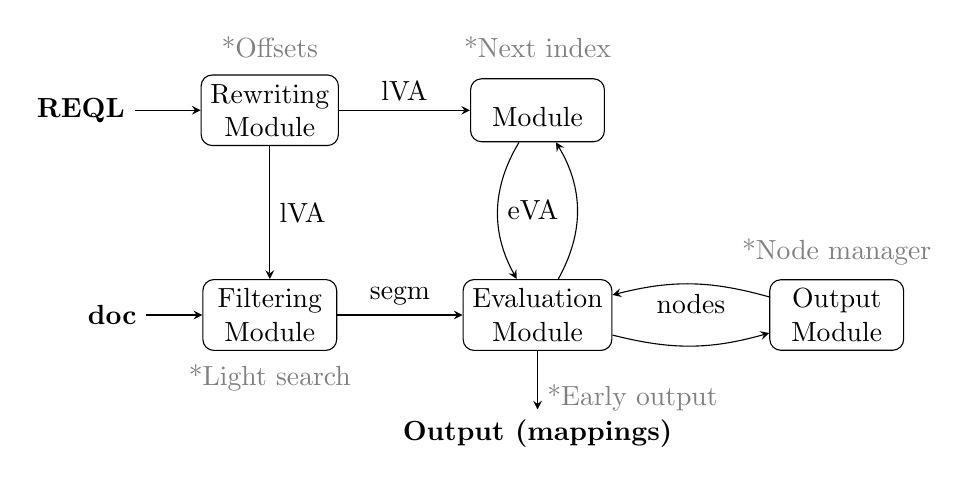
\begin{tikzpicture}[
	every text node part/.style={align=center}]	
	
	\tikzstyle{mmodule}=[rectangle, draw=black, fill=white, minimum height=8mm, minimum width=1.7cm, rounded corners]
	\tikzstyle{medge} = [->,>=stealth,auto]	
	\tikzstyle{opt} = [black!50]
	
	%\draw[step=.5cm, dashed, draw=black!20] (-1,-1) grid (8,3);
	
	\node [mmodule] (rmod) at (1, 2) {Rewriting \\ Module};
	
	\node [mmodule, below of=rmod,node distance=2.6cm] (fmod) {Filtering \\ Module};
	
	\node [mmodule, right of=rmod, node distance=3.4cm] (detmod) {$\cdet$ \\ Module};
	
	\node [mmodule, below of=detmod, node distance=2.6cm] (evalmod) {Evaluation \\ Module};
	
	\node [mmodule, right of=evalmod, node distance=3.8cm] (nodman) {Output \\ Module};
	
	\node[left of=rmod, node distance=2.4cm] (REQL) {\textbf{REQL}};
	
	\node[left of=fmod, node distance=2cm] (doc) {\textbf{doc}};
	
	\node[below of=evalmod, node distance=1.5cm] (output) {\textbf{Output (mappings)}};
	
	\draw[medge] (REQL) edge (rmod); 
	
	\draw[medge] (doc) edge (fmod); 
	
	\draw[medge] (rmod) edge node {lVA} (detmod);
	
	\draw[medge] (rmod) edge node {lVA} (fmod);
	
	\draw[medge] (detmod) edge[bend right] node {eVA} (evalmod);
	\draw[medge] (evalmod) edge[bend right] (detmod);
	
	\draw[medge] (fmod) edge node {segm} (evalmod);
	
	\draw[medge] (nodman) edge[bend right=15] node {nodes} (evalmod);
	\draw[medge] (evalmod) edge[bend right=15] (nodman);
	
	\draw[medge] (evalmod) edge node[opt, pos=0.8] {*Early output} (output); 
	
	\node[opt,above of=rmod, node distance=0.8cm] {*Offsets};
	
	\node[opt,below of=fmod, node distance=0.8cm] {*Light search};
	
	\node[opt,above of=nodman, node distance=0.8cm] {*Node manager};
	
	\node[opt,above of=detmod, node distance=0.8cm] {*Next index};
	
%	\node [state] (n0) at (0,0) {$\bot$};
%	
%	\node [state] (n1) at ($(n0)+(1.3,-1)$) {$[x,\!0$};
%	\node [state] (n2) at ($(n0)+(1.3,0)$) {$[x,\!3$};
%	\node [state] (n3) at ($(n0)+(1.3,1)$) {$[x,\!6$};
%	
%	\node [state] (n9) at ($(n0)+(0,1)$) {$[x,\!9$};
%	
%	\node [state] (n4) at ($(n2)+(1.3,-1)$) {$x\rangle,\!4$};
%	\node [state] (n5) at ($(n2)+(1.3,0)$) {$x\rangle,\!7$};
%	\node [state] (n6) at ($(n2)+(1.3,1)$) {$x\rangle,\!10$};
%	
%	\node [state] (n7) at ($(n4)+(1.3,0)$) {$\cup$};
%	
%	\node [state] (n8) at ($(n7)+(1.3,1)$) {$\cup$};
%	
%	\draw[<-] (n0) to (n1);
%	\draw[<-] (n0) to (n2);
%	\draw[<-] (n0) to (n3);
%	
%	\draw[<-] (n1) to (n4);
%	\draw[<-] (n2) to (n5);
%	\draw[<-] (n3) to (n6);
%	
%	\draw[<-] (n4) to (n7);
%	\draw[<-] (n5) to (n7);
%	
%	\draw[<-] (n7) to (n8);
%	\draw[<-] (n6) to (n8);
%	\draw[<-] (n0) to (n9);

\end{tikzpicture}
	\caption{Architecture of \rematch. Optimizations are marked with * and in grey. lVA stands for Logical VA, eVA for Extended VA, and segm for segments.}
	\label{fig:architecture}
\end{figure}

\section{Experimental setup}
\label{ss:setup}

\subsection{The implementation}
\rematch\ was implemented in C++, and includes all the components presented in
the thesis. An overview of the \rematch\ architecture can be found in
Figure~\ref{fig:architecture}. Each module was described in a chapter of the
thesis. The Rewriting module (Chapter~\ref{chpt:rewriting}) takes a REQL
expression and converts it to a logical VA, which is used both by the
\textsf{DET} module (Chapter~\ref{chpt:evaluation}), and by the Filtering module
(Chapter~\ref{chpt:filtering}). The latter processes the input document by
splitting it into segments containing outputs, which are then passed to the
Evaluation module (Chapter~\ref{chpt:evaluation}). The Evaluation module runs
Algorithm~\ref{alg:evaluation} by communicating with the \textsf{DET} module to
obtain the next state of the eVA, and with the Output module
(Chapter~\ref{chpt:output}), which creates the nodes of the data structure
encoding the output mappings. Specific optimizations were highlighted in each
chapter.


\subsection{The datasets}
We use the following three real-world text corpora:
\begin{enumerate}
	\item \textsf{Literature.}  This is a combined corpus of collected works by
	Mark Twain, William Shakespeare, and Charles Dickens. We used texts provided
	by Project Gutenberg\footnote{\url{https://www.gutenberg.org/}}, and
	concatenated them into a single document of size 50.7 MB ( around 50 million
	characters).
	\item \textsf{DNA.} This dataset consists of DNA sequences. In particular,
	we used the list of proteomes of the zebrafish organism that is provided by
	the BLAST
	initiative\footnote{\url{https://blast.ncbi.nlm.nih.gov/doc/blast-help/downloadblastdata.html}}.
	The combined size of this dataset is 38.5 MB (around 38 million characters).
	\item \textsf{SPARQL.} Our final dataset consists of public query logs of
	the (now defunct) British Museum SPARQL endpoint, as extracted and collected
	by the Linked SPARQL Queries Dataset
	team\footnote{\url{http://aksw.github.io/LSQ/}}. We merged all the logs into
	a single document weighing 71.1 MB, and consisting of roughly 76 million
	characters.
\end{enumerate}

\subsection{The queries}
Our queries for each dataset are designed as follows:
\begin{enumerate}
	\item \textsf{Literature.} Here we take a list of common English language
	morphemes\footnote{A morpheme is the smallest meaningful constituent of a
	linguistic expression, \url{https://en.wikipedia.org/wiki/Morpheme}.}, as
	provided by~\citet{morphemes}. We then specify queries that look for
	2-grams~\citep{morphemes}, that is, two consecutive words each containing a
	morpheme from our list (e.g. the first word ends in -ing, and the second one
	in -er).
	\item \textsf{DNA.} Motif detection is a key task in DNA
	analysis\footnote{\url{https://en.wikipedia.org/wiki/Sequence_motif}}. In
	this query set we select 100 DNA motifs from the Prosite
	database~\citep{prosite} that commonly occur in our dataset. Our queries
	take any such pair of motifs, and look for their occurrences in the
	proteomic sequence separated by at most 20 characters.
	\item \textsf{SPARQL.} Our  logs have distinct SPARQL queries listed in each
	line. For our expressions we fix two sets of up to three SPARQL
	keywords~\citep{sparql11} (e.g., \texttt{WHERE} or \texttt{OPTIONAL}), and
	extract two consecutive queries where the first one contains the keywords
	from the first set, and the second one from the second set. 
\end{enumerate}

For each dataset roughly 10,000 queries were generated. We then sample 150
queries from each set and use these for our experiments, this in order to reduce
the overall experimentation time to gather results. The queries were designed
such they cover real world-scenarios where overlapping matches occur naturally.
For instance, in the \textsf{DNA} dataset, a starting motif might be paired with
multiple occurrences of an end motif, which is a natural use case for the
all-match semantics, and something that is difficult to capture using modern
RegEx engines, as shown in Table~\ref{tab:outputs}. 


\subsection{How we ran the queries}
All the experiments were run on a Apple M1 Pro 10 cores/10 threads machine with
clock speed 2064 -- 3220 MHz and 16GB RAM. The operating system used was MacOS
13.1.   The \rematch\ implementation binary was compiled using \texttt{clang}
with code optimization (\texttt{-O3} flag). Queries were run in succession, and
each query was executed 5 times. We collected the average runtime and memory
consumption of each query, and consider these in our measurements.

\section{What do our optimizations do?}\label{ss:internal} Throughout the thesis
we described a series of optimizations which define the \rematch\ system
architecture, as illustrated in Figure~\ref{fig:architecture}. Of course, a
natural question to ask is what is the effect of each one of these
optimizations, and whether implementing the basic algorithm for computing all
matches of a REQL expression  would be competitive enough already? In this
section, we test that hypothesis, and show that a vanilla implementation of
Algorithm~\ref{alg:evaluation} runs several orders of magnitude slower that the
full \rematch\ stack. Additionally, we test how each single optimization affects
the performance of \rematch.




For this, we run the experiments described in Section~\ref{ss:setup}, and test
the following versions of \rematch:
\begin{itemize}
	\item \textsc{Naive}, which is just the implementation of
	Algorithm~\ref{alg:evaluation}.
	\item \textsc{Node Manager}, which adds the $\ds$ module to discard unusable
	nodes as soon as possible (Chapter~\ref{chpt:output}).
	\item \textsc{Next Index}, which uses an ASCII character table in the
	automaton transitions for quick access (Chapter~\ref{chpt:evaluation}).
	\item \textsc{Offset}, which postpones storing the (potential) output
	information as much as possible (Chapter~\ref{chpt:rewriting}).
	\item \textsc{Early Output}, which outputs results as soon as they are
	available (Chapter~\ref{chpt:output}).
	\item \textsc{Light Search}, which finds a valid segmentation of the
	document that are guaranteed to produce the output and runs the full
	algorithm over these segments (Chapter~\ref{chpt:filtering}).
\end{itemize}

Here each new version includes all the optimizations  previously listed. For
example, the \textsc{Offset} version of the algorithm includes both the
\textsc{Node Manager} and the \textsc{Next index} optimizations. As the
optimizations are designed to help the algorithm in various aspects, we test
their impact along three dimensions: (i) time; (ii) memory consumption; and
(iii) time needed to return the first output. Boxplots for time and first output
time are presented in Figures \ref{fig:opt-time} and \ref{fig-optimizations},
while Table~\ref{tab-memory} shows the average memory consumption.


\begin{figure}[t]
	\centering
	\centering
	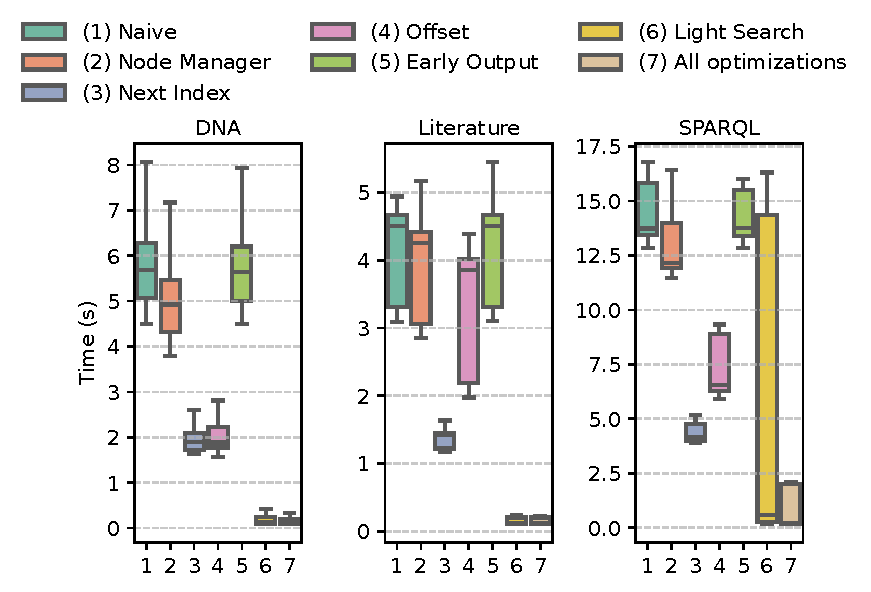
\includegraphics[width=.8\textwidth]{figures/versions-time.pdf}
	\caption{Runtime performance of \rematch\ optimizations}
	\label{fig:opt-time}
\end{figure}

\begin{figure}[t]
	\centering
	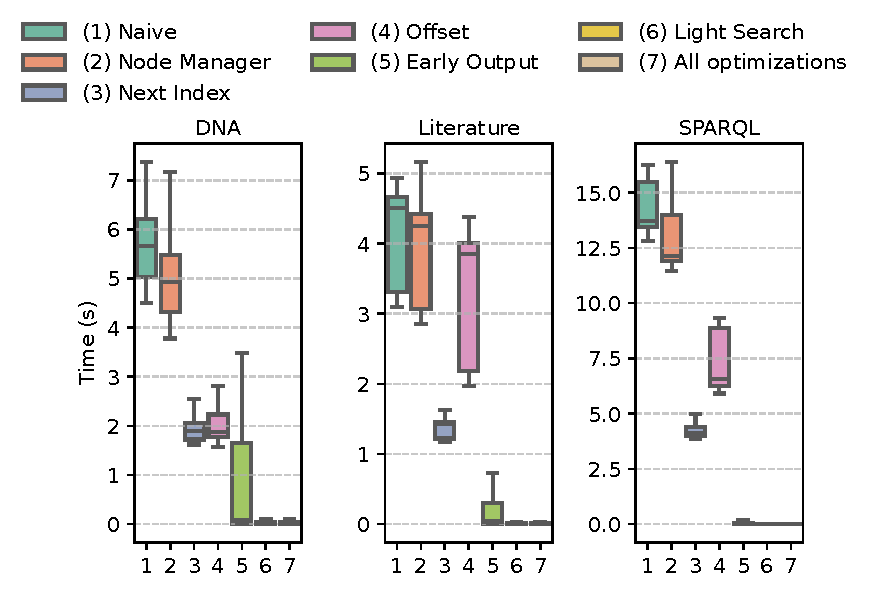
\includegraphics[width=.8\textwidth]{figures/versions-fot.pdf}
	\label{fig:opt-firstOT}
	\caption{Time to produce the first output of \rematch\ optimizations}
	\label{fig-optimizations}
\end{figure}

% TODO: Gonzalo says that Offset and Early Output worsen things. Asks if we
% tried to run Light Search without them.


\subsection{Discussion}
As we can observe (Figure~\ref{fig:opt-time}), among all three datasets, adding
the \textsc{Node Manager} module makes the runtime of our experiments drop
noticeably, however the real savings come from the \textsc{Next index}
optimization, which allows us to instantaneously check whether a character
triggers an automaton transition. The \textsc{Offset} and \textsc{Light Search}
version reduces the runtime in a meaningful manner as well. Concerning memory
consumption (Table~\ref{tab-memory}), \textsc{Node Manager} drastically reduces
the memory consumption compared to the \textsc{Naive} version. Due to storing
more information in each transition, \textsc{Next index} increases memory
consumption, and \textsc{Offset} and \textsc{Early Output} tend to decrease it
again due to discarding nodes that are not needed any more by the algorithm
sooner. Considering time to first output (Figure~\ref{fig-optimizations}), we
can see that \textsc{Next index} drops the runtime by an order of magnitude, and
another order of magnitude is gained by \textsc{Early Output}, whose main
objective is precisely this: deliver the outputs to the user as soon as
possible. Overall, our experiments show that the proposed optimizations, which
are closely linked to the \rematch\ architecture
(Figure~\ref{fig:architecture}), indeed improve the performance of base
algorithm, denoted \textsc{Naive}, by orders of magnitude.


\begin{table}[t]
	\begin{tabular}{l|rrr}
		                      & \textsf{DNA} & \textsf{Literature} &
		                      \textsf{SPARQL} \\
		\hline
		\textsc{Naive}        & 823.30        & 379.90               & 1229.69
		\\
		\textsc{Node Manager} & 6.08         & 2.10                 & 8.75 \\
		\textsc{Next Index}   & 18.32        & 2.33                & 10.10 \\
		\textsc{Offset}       & 18.66        & 2.32                & 7.78 \\
		\textsc{Early Output} & 16.09        & 2.21                & 3.64 \\
		\textsc{Light Search} & 23.36        & 2.09                & 3.87
	\end{tabular}
	\caption{Average memory usage of \rematch\ versions (in MB).}
	\label{tab-memory}
\end{table}

\section{Comparison with other engines}\label{ss:comp}


\subsection{The setup}
Here we do a thorough analysis of how \rematch\ compares to classic RegEx
processing libraries. For this, we tried to be thorough, and include both
engines that can approximate the all-match semantics using look-around
operators, and others that cannot. In our comparison the following engines are
used:
\begin{itemize}
	\item \textsf{PCRE}~\citep{pcre} version: 8.45;
	\item \textsf{PCRE2}~\citep{pcre2} version 10.40 (using JPCRE2 C++
	wrapper~\citep{wrapper});
	\item \textsf{Boost.Regex}~\citep{boost} version 1.81.0;
	\item \textsf{Oniguruma}~\citep{oniguruma} version 6.9.7.1;
	\item \textsf{RE2}~\citep{re2} version 2021--11--01; and
	\item \textsf{TRE}~\citep{tre} version 0.8.0.
\end{itemize}
For engines that support look-around operators (\textsf{PCRE}, \textsf{PCRE2},
\textsf{Boost} and \textsf{Oniguruma}) we rewrite the experiments from
Section~\ref{ss:setup} so that they retrieve all the matches. For \textsf{RE2}
and \textsf{TRE}, which do not support look-around operators, we rewrite the
queries using capture groups such they resemble as closely as possible the
original experiments, although they do not perform the same task.


The results are presented in Figure~\ref{fig:comparison} and
Table~\ref{tab:outputs}. Here we compare only in terms of time. The memory
consumption was relatively stable along all the engines, with \rematch\ using
the most memory, but only by a negligible amount (kilobytes in our experiments),
which is justified by the extra bookkeeping done by \rematch\ in order to
retrieve all the matches.  \rematch\ had some spikes in memory usage for the
\textsf{DNA} dataset, and \textsf{PCRE2} in the \textsf{SPARQL} dataset, but the
document size still dominated memory usage significantly.

In this discussion, it is essential to recall that REmatch is incomparable with
standard RegEx engines, given that it uses a different query language for always
finding all matches (even DNA queries with look-around provide less number of
outputs). Then it is not our purpose here to prove that REmatch is ``faster''
than other RegEx engines. Quite the opposite, we want to test that, although
REmatch is running a more heavy processing task, the performance is comparable
to the standard and highly optimized RegEx engines.

\begin{table}
	\begin{tabular}{l|ccc}
		                   & \textsf{DNA}      & \textsf{Literature} &
		                   \textsf{SPARQL}   \\
		\hline
		\rematch           & \textbf{16,187.4} & \textbf{706.6}      &
		\textbf{29,424.2} \\
		\textsf{RE2}       & 10,556.9          & 704.9               & 12,287.8
		\\
		\textsf{PCRE}      & 13,130.4          & 705.1               &
		\textbf{29,424.2} \\
		\textsf{PCRE2}     & 13,130.4          & 705.1               &
		\textbf{29,424.2} \\
		\textsf{Boost}     & 13,130.4          & 642.6               &
		\textbf{29,424.2} \\
		\textsf{Oniguruma} & 13,130.4          & 705.5               &
		\textbf{29,424.2} \\
		\textsf{TRE}       & 10,556.9          & 704.2               & N/A
	\end{tabular}
	\caption{Average number of outputs (highest in bold).}
	\label{tab:outputs}
\end{table}

\begin{figure}[t]
	\centering
	\begin{subfigure}[b]{.8\textwidth}
		\centering
		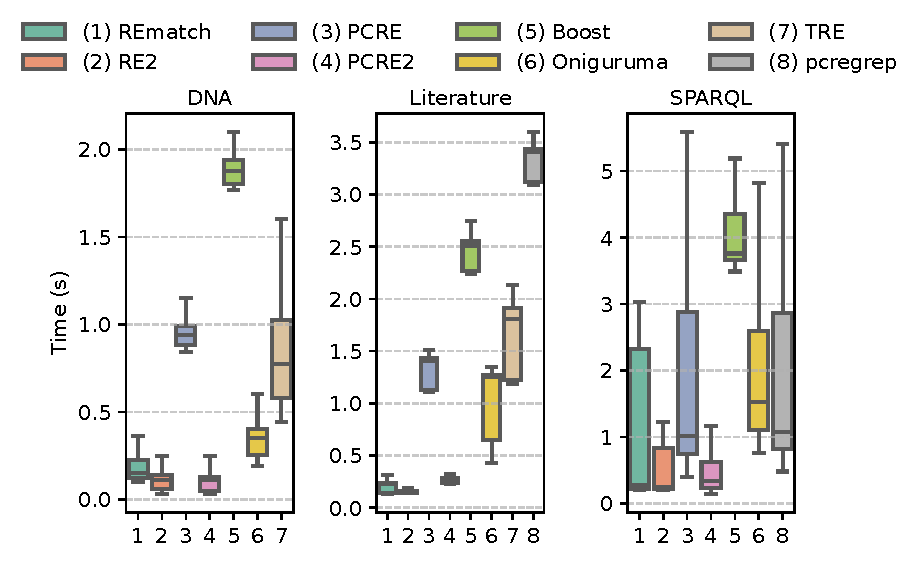
\includegraphics[width=\textwidth]{figures/lookahead-time.pdf}
	\end{subfigure}
	\caption{Runtime metrics of our experiments}
	\label{fig:comparison}
\end{figure}



\subsection{Discussion}
As we can see from Figure~\ref{fig:comparison}, \rematch\ shows good performance as compared to other engines. On
the \textsf{Literature} dataset, \rematch\ is bested only by \textsf{RE2}, which
does not look for all the outputs. On the \textsf{DNA} dataset \rematch\ is a
close third, bested only by \textsf{RE2} and \textsf{PCRE2} by a tiny margin.
In regards to \textsf{SPARQL}, the analysis is similar. We remark that in this
dataset \textsf{TRE} throws an error on every query. Comparing the number of
outputs, in Table~\ref{tab:outputs} we can observe that \rematch\ generally does
more work compared to other engines. This is particularly evident when comparing
to engines not using look-around operators (\textsf{RE2} and \textsf{TRE}). Even
for the engines with look-around supported, we sometimes cannot capture all the
outputs (for instance when two nested matches start at the same position), as
witnessed in Table~\ref{tab:outputs}. Overall, the experiments illustrate that
the task of encountering \emph{all} the outputs, including overlapping ones, can
be done with minimal overhead when comparing with classical RegEx matching.
